%!TEX root = ../paper.tex
We compare the performance of the Modified Breiman Estimator with isotropic and anisotropic kernels on simulated data sets with known density fields. This allows us to test how well the shape-adaptive method recovers simple density distributions in comparison to the fixed-shape method.
% Which metrices do we use
The \mse (\MSE) is used to quantify the performance of the estimators. We use
\begin{equation*}\label{eq:experiment:anisotropicmetric}
	\frac{\max\left(\varEigenValue_1, \dotsc, \varEigenValue_\varDim \right)}{\min\left(\varEigenValue_1, \dotsc, \varEigenValue_\varDim \right)}
\end{equation*}
where $\varEigenValue_1, \dotsc, \varEigenValue_\varDim$ are the eigenvalues of the bandwidth matrix, to express how anisotropic a kernel is.
%Quickly introduce the datasets
Two different types of data sets are used: data sets consisting of a single Gaussian distribution with an uniform random background, defined in \cref{s:experiment:singlesphere},  and data sets containing multiple Gaussian distributions embedded in an uniform distribution, which are presented in \cref{s:experiment:multisphere}.

\begin{figure*}
	\centering
	%!TEX root = ../../paper.tex

%Ferdosi Sets 1
\begin{subfigure}{0.23\textwidth}
	\centering
	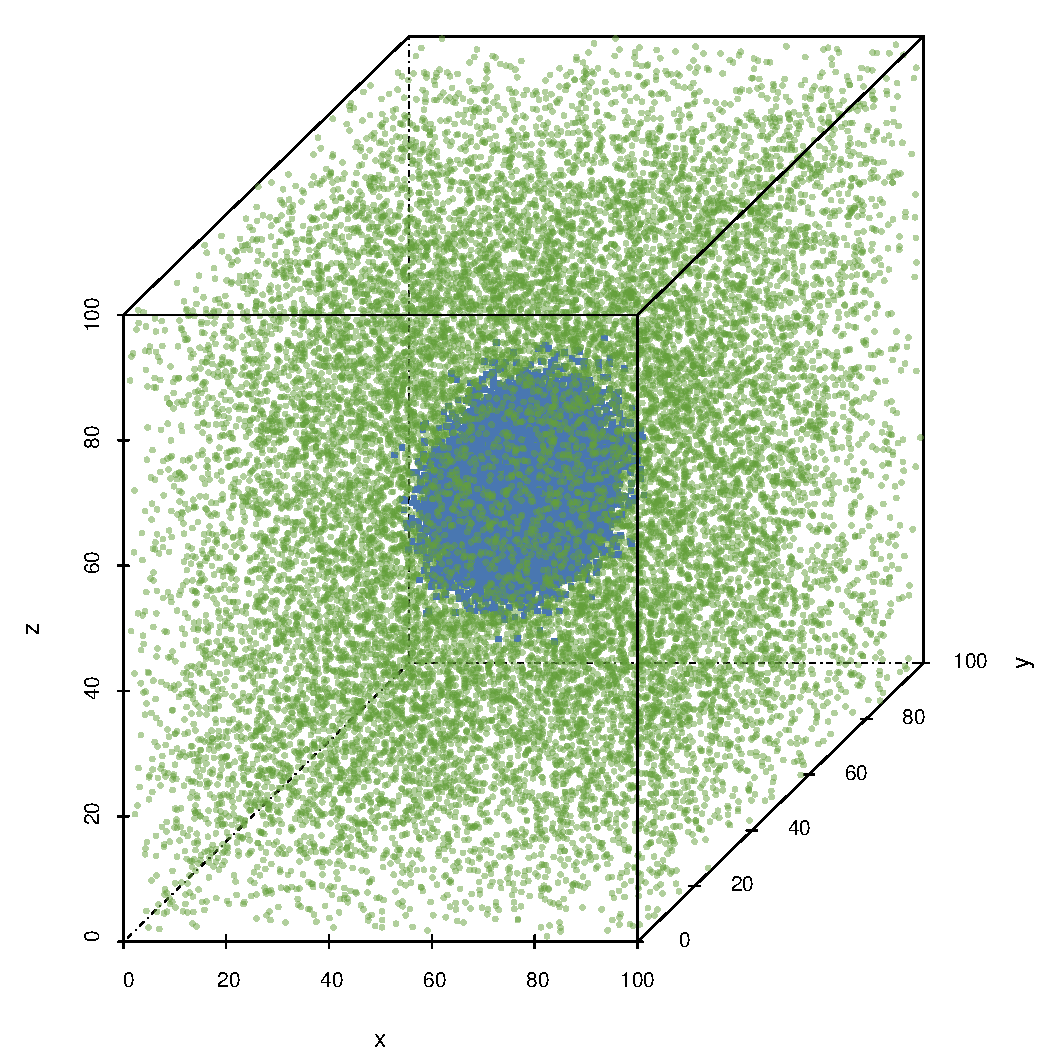
\includegraphics[width=\textwidth]{experiment/img/datasetplot_ferdosi_1_60000}
	\caption{Set \ferdosiOne}
	\label{fig:experiment:singlesphere:ferdosi1}
\end{subfigure}
% Baakman 1	
\begin{subfigure}{0.23\textwidth}
	\centering
	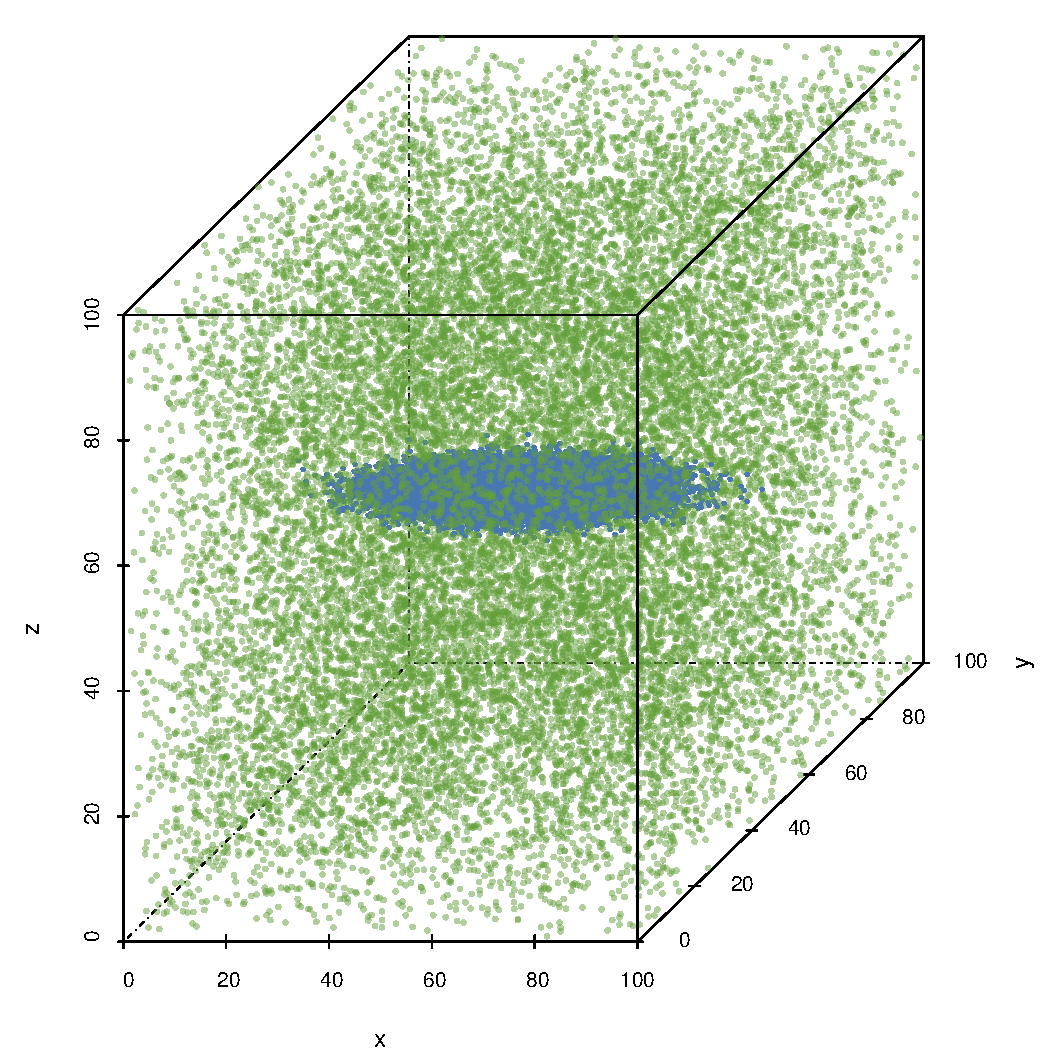
\includegraphics[width=\textwidth]{experiment/img/datasetplot_baakman_1_60000}
	\caption{Set \baakmanOne}
	\label{fig:experiment:singlesphere:baakman1}
\end{subfigure}
% Baakman 4
\begin{subfigure}{0.23\textwidth}
	\centering
	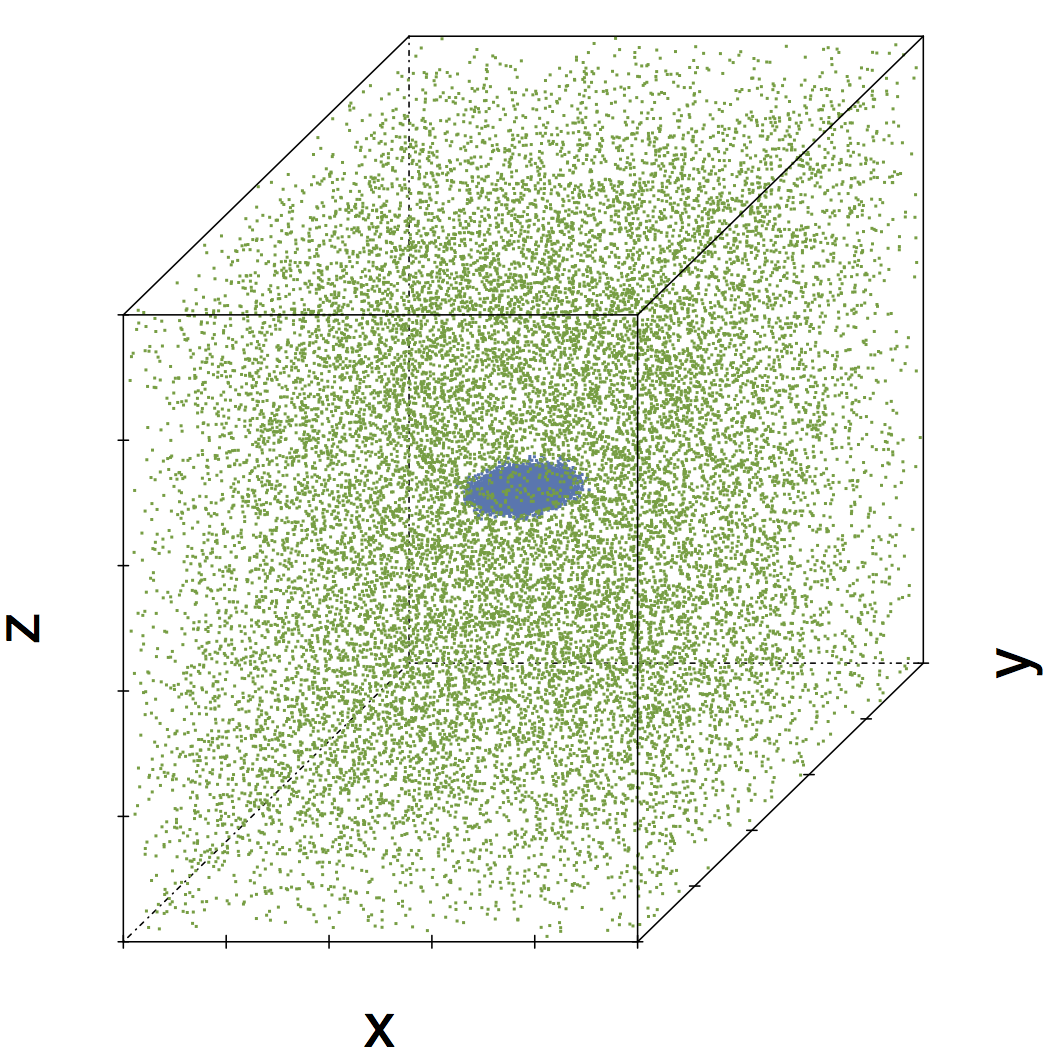
\includegraphics[width=\textwidth]{experiment/img/datasetplot_baakman_4_60000}
	\caption{Set \baakmanFour}
	\label{fig:experiment:singlesphere:baakman4}
\end{subfigure}	
% Baakman 5
\begin{subfigure}{0.23\textwidth}
	\centering
	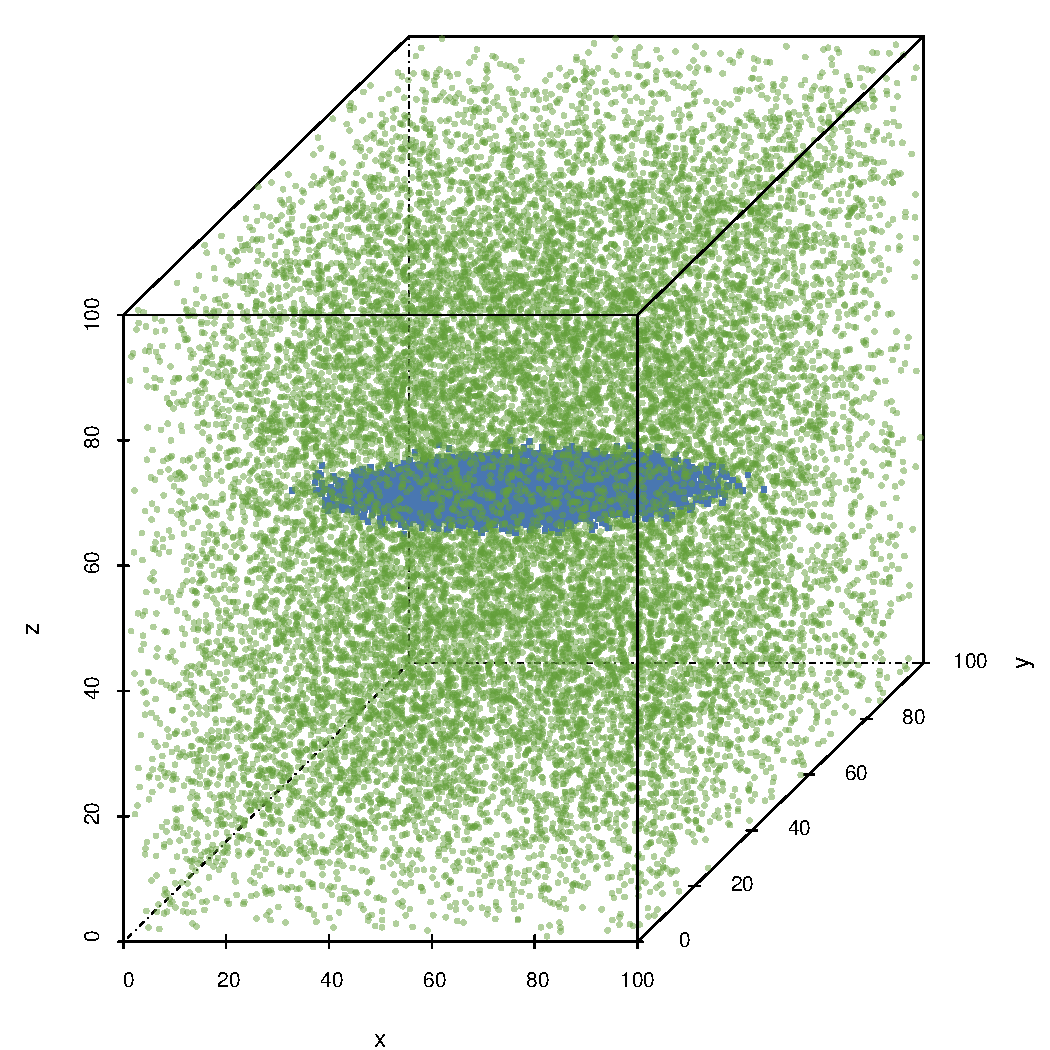
\includegraphics[width=\textwidth]{experiment/img/datasetplot_baakman_5_60000}
	\caption{Set \baakmanFive}
	\label{fig:experiment:singlesphere:baakman5}
\end{subfigure}	
	\caption{Scatter plot representation of the data sets with a single Gaussian, defined in \cref{tab:experiment:singlesphere:sets}. The used colors correspond to those associated with the different components in \cref{tab:experiment:singlesphere:sets}.}
	\label{fig:experiment:singlesphere:sets}
\end{figure*}

\begin{table*}
	\centering
	%!TEX root = ../../paper.tex
\small
\sisetup{
	table-format=5.0,
	scientific-notation=false,
	round-mode=places,
	round-precision=1,
	table-number-alignment=center
}
\begin{tabular}{@{}cclSl@{}}
\toprule
				&~						& Component					& {Samples} 	& Distribution\\
\midrule
% Ferdosi 1
\ferdosiOne 	&\legendComponentOne	& Trivariate Gaussian 		& 40000		& $\gaussDist{[50, 50, 50]}{\diag(11)}$\\
~ 				&\legendComponentNoise	& Uniform random background	& 20000		& $\uniformDist{[0, 0, 0]}{[100, 100, 100]}$\\
% Baakman 1
\hline
\baakmanOne		&\legendComponentOne	& Trivariate Gaussian 		& 40000		& $\gaussDist{[50, 50, 50]}{\diag([11^2, \sqrt{11}, \sqrt{11}])}$\\
~ 				&\legendComponentNoise	& Uniform random background	& 20000		& $\uniformDist{[0, 0, 0]}{[100, 100, 100]}$\\
% Baakman 4
\hline
\baakmanFour	&\legendComponentOne	& Trivariate Gaussian 		& 40000		& $\gaussDist{[50, 50, 50]}{\diag([11, 2 * \sqrt{11}, \rfrac{1}{2} \sqrt{11}])}$\\
~ 				&\legendComponentNoise	& Uniform random background	& 20000		& $\uniformDist{[0, 0, 0]}{[100, 100, 100]}$\\
% Baakman 5
\hline
\baakmanFive	&\legendComponentOne	& Trivariate Gaussian 		& 40000		& $\gaussDist{[50, 50, 50]}{\diag([11^2, 11, 1])}$\\
~ 				&\legendComponentNoise	& Uniform random background	& 20000		& $\uniformDist{[0, 0, 0]}{[100, 100, 100]}$\\
\bottomrule
\end{tabular}
	\caption{The data sets with multiple Gaussian distributions embedded in uniform random background. This table has the same structure and uses the same notation as \cref{tab:experiment:singlesphere:sets}.}
	\label{tab:experiment:multisphere:sets}
\end{table*}

\subsection{Data Sets with a Single Gaussian}
\label{s:experiment:singlesphere}
%!TEX root = ../../paper.tex

This section compares the performance of the Modified Breiman Estimator with symmetric and shape-adaptive kernels on data sets that contain one Gaussian component.
%MSE
	\begin{table}
		\centering
		%!TEX root = ../../paper.tex

\begin{tabular}{l*{2}{S[scientific-notation=true, round-mode=places,round-precision=3]}}
\toprule
~ 				& \multicolumn{2}{c}{Estimator}\\ \cmidrule{2-3}
Set				& {\mbe}					& {\sambe}	\\
\midrule
\ferdosiOne		& 8.30580618349064E-09		&  8.9087329457441E-09 \\
\baakmanOne		& 1.49022877061299E-08		&  1.5398737157543E-08 \\	
\baakmanFour	& 2.93709420107411E-08		&  2.9634323205557E-08 \\	
\baakmanFive	& 5.57179476550916E-08		&  5.5847473903432E-08 \\	
\bottomrule
\end{tabular}
		\caption{\Mses of the estimator with fixed-shape (\mbe) and shape-adaptive (\sambe) kernels on data set \ferdosiOne through \baakmanFive.}
		\label{tab:results:singleSphere:mse}
	\end{table}
	%
	Comparing the \mses of the \mbe with those of \sambe in \cref{tab:results:singleSphere:mse} we find that the estimators perform comparably, but that the fixed-shape estimator consistently gives a slightly lower \mse.

%PLOTS
	\begin{figure*}
		\centering
		%!TEX root = ../../paper.tex

% Ferdosi 1 - MBE
\begin{subfigure}{0.3\textwidth}
	\centering
	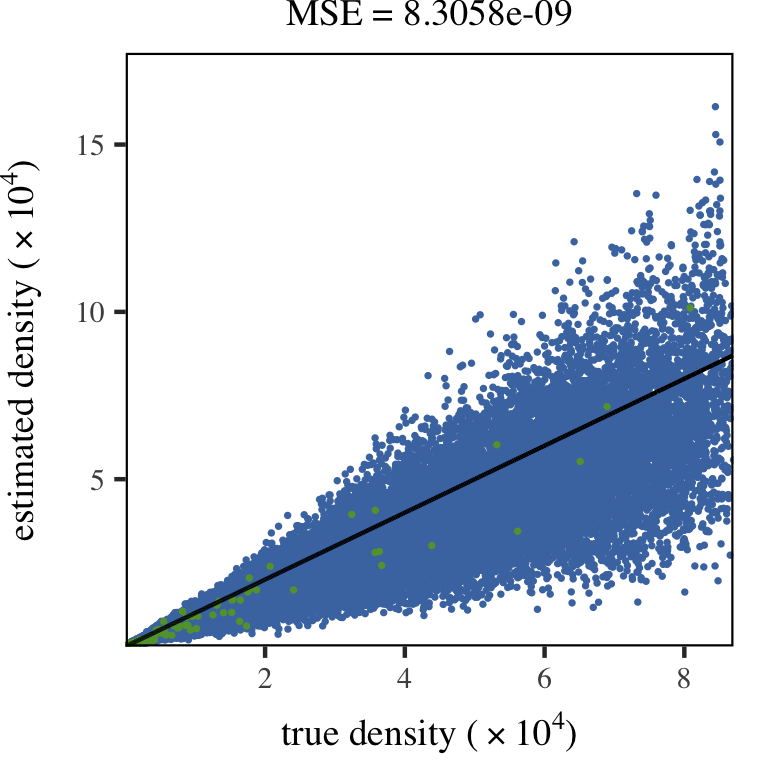
\includegraphics[keepaspectratio=true, width=\textwidth, height=0.23\textheight]{result/img/results_ferdosi_1_60000_mbe_silverman}
	\caption{Set \ferdosiOne, \mbe}
	\label{fig:results:singlesphere:mbe:ferdosi1}
\end{subfigure}
% Ferdosi 1 - SAMBE
\begin{subfigure}{0.3\textwidth}
	\centering
	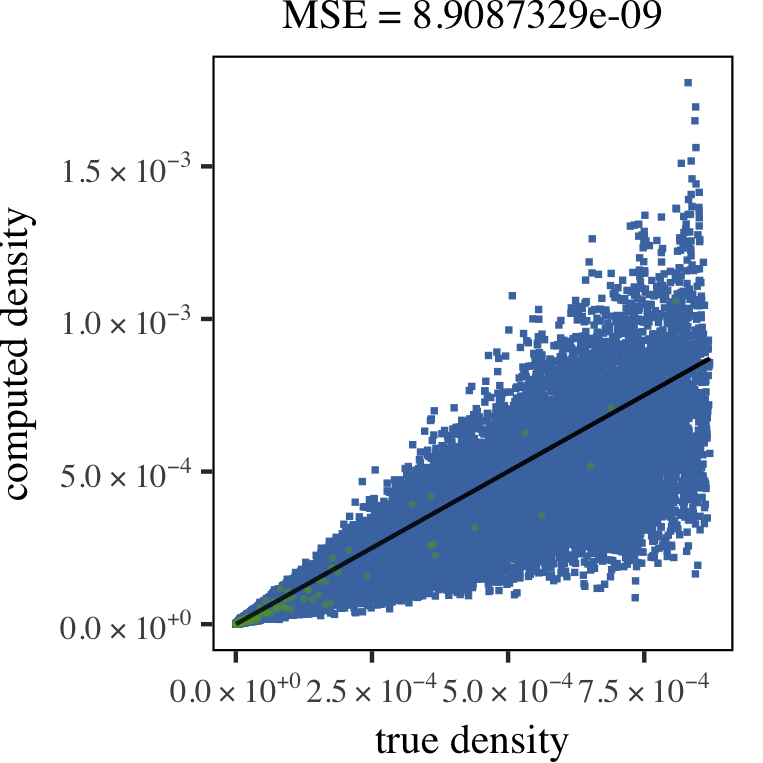
\includegraphics[keepaspectratio=true, width=\textwidth, height=0.23\textheight]{result/img/results_ferdosi_1_60000_sambe_silverman}
	\caption{Set \ferdosiOne, \sambe}
	\label{fig:results:singlesphere:sambe:ferdosi1}
\end{subfigure}
\subfigvspace
% Baakman 1	- MBE
\begin{subfigure}{0.3\textwidth}
	\centering
	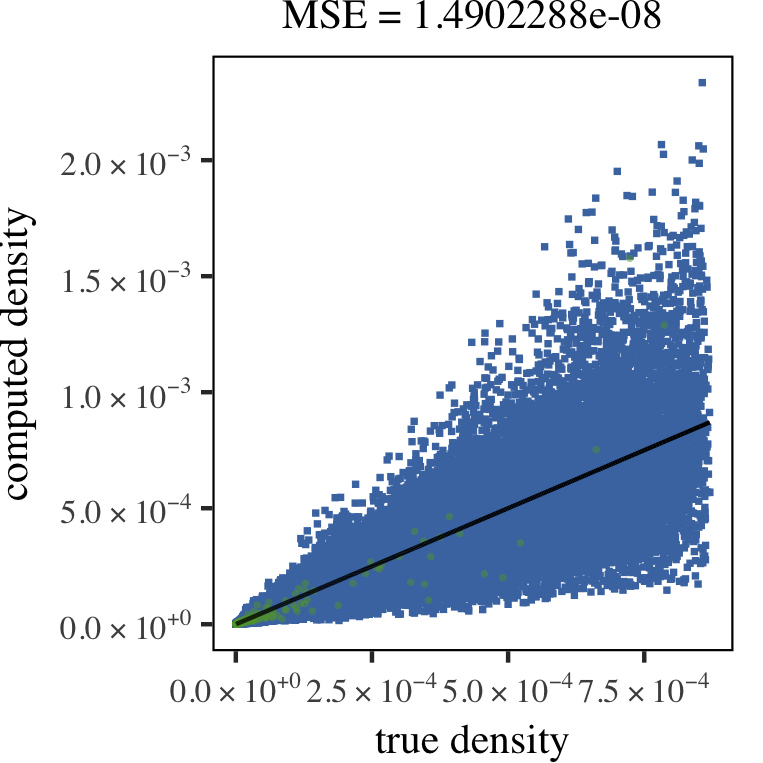
\includegraphics[keepaspectratio=true, width=\textwidth, height=0.23\textheight]{result/img/results_baakman_1_60000_mbe_silverman}
	\caption{Set \baakmanOne, \mbe}
	\label{fig:results:singlesphere:mbe:baakman1}
\end{subfigure}
% Baakman 1	- SAMBE
\begin{subfigure}{0.3\textwidth}
	\centering
	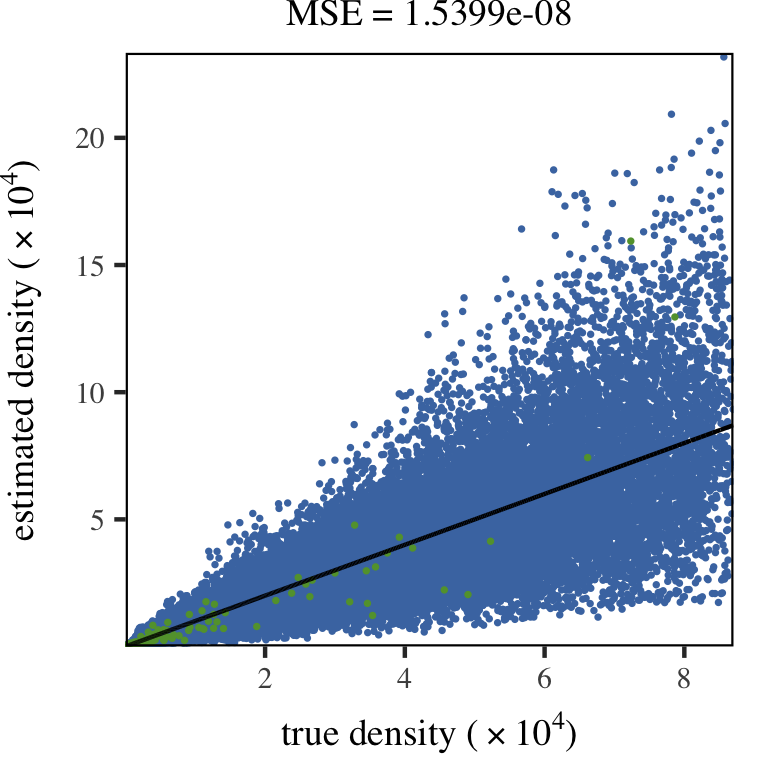
\includegraphics[keepaspectratio=true, width=\textwidth, height=0.23\textheight]{result/img/results_baakman_1_60000_sambe_silverman}
	\caption{Set \baakmanOne, \sambe}
	\label{fig:results:singlesphere:sambe:baakman1}
\end{subfigure}
\subfigvspace
% Baakman 4 - MBE
\begin{subfigure}{0.3\textwidth}
	\centering
	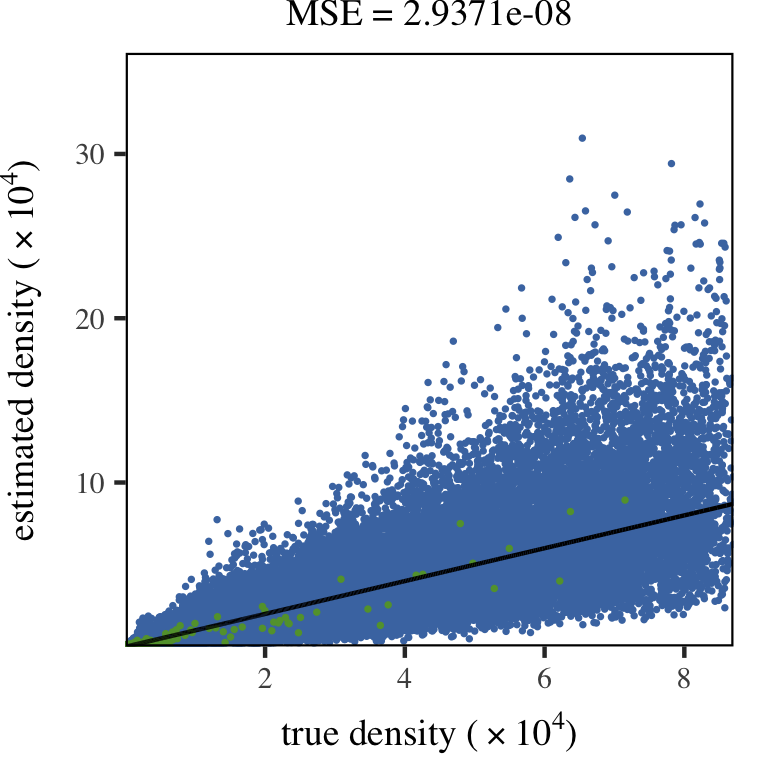
\includegraphics[keepaspectratio=true, width=\textwidth, height=0.23\textheight]{result/img/results_baakman_4_60000_mbe_silverman}
	\caption{Set \baakmanFour, \mbe}
	\label{fig:results:singlesphere:mbe:baakman4}
\end{subfigure}	
% Baakman 4 - SAMBE
\begin{subfigure}{0.3\textwidth}
	\centering
	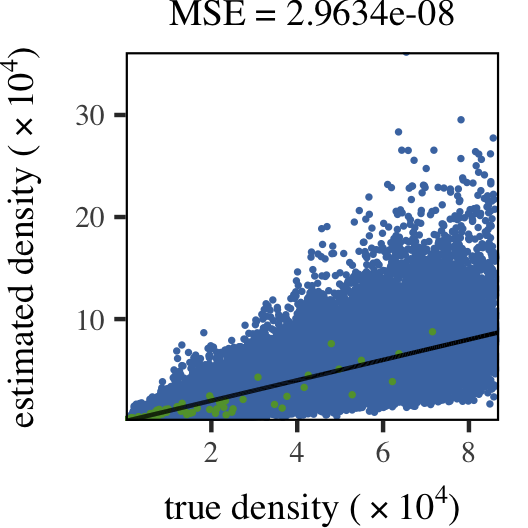
\includegraphics[keepaspectratio=true, width=\textwidth, height=0.23\textheight]{result/img/results_baakman_4_60000_sambe_silverman}
	\caption{Set \baakmanFour, \sambe}
	\label{fig:results:singlesphere:sambe:baakman4}
\end{subfigure}		
\subfigvspace
% Baakman 5 - MBE
\begin{subfigure}{0.3\textwidth}
	\centering
	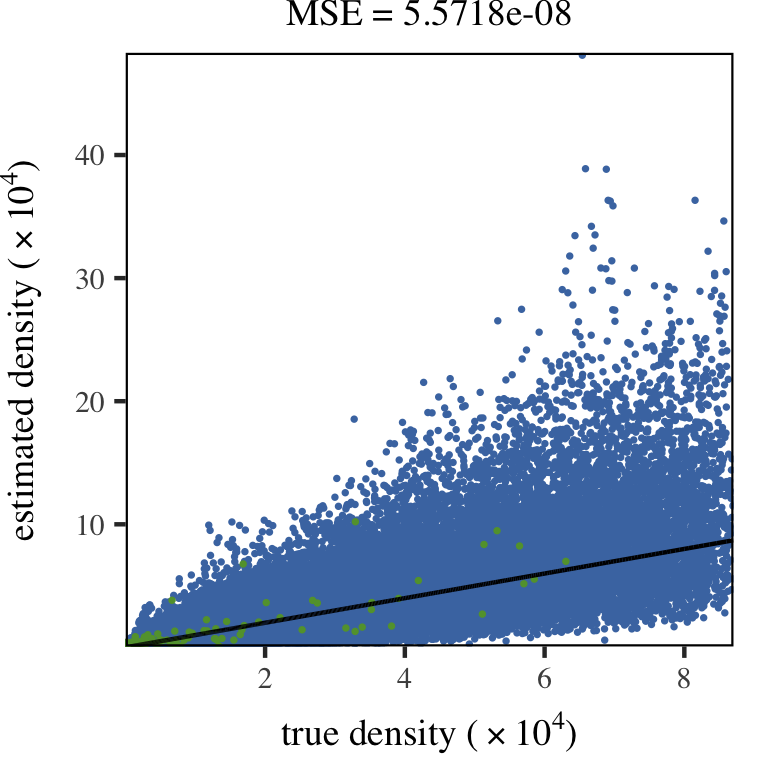
\includegraphics[keepaspectratio=true, width=\textwidth, height=0.23\textheight]{result/img/results_baakman_5_60000_mbe_silverman}
	\caption{Set \baakmanFive, \mbe}
	\label{fig:results:singlesphere:mbe:baakman5}
\end{subfigure}
% Baakman 5 - SAMBE
\begin{subfigure}{0.3\textwidth}
	\centering
	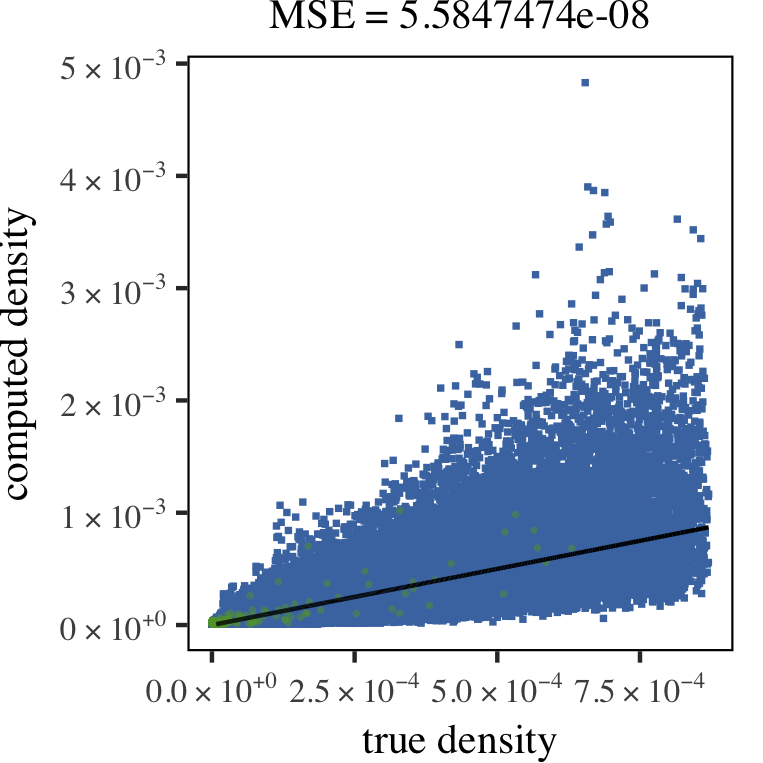
\includegraphics[keepaspectratio=true, width=\textwidth, height=0.23\textheight]{result/img/results_baakman_5_60000_sambe_silverman}
	\caption{Set \baakmanFive, \sambe}
	\label{fig:results:singlesphere:sambe:baakman5}
\end{subfigure}	
		\caption{The density as estimated by \mbe and \sambe as a function of the known density of data sets \ferdosiOne through \baakmanFive.}
		\label{fig:results:singleSphere:comparativePlots}
	\end{figure*}
	%
	This is confirmed by the visualization of the results in \cref{fig:results:singleSphere:comparativePlots} where hardly any difference is visible between \cref{fig:results:singlesphere:mbe:ferdosi1,fig:results:singlesphere:mbe:baakman1,fig:results:singlesphere:mbe:baakman4,fig:results:singlesphere:mbe:baakman5}, and \cref{fig:results:singlesphere:sambe:ferdosi1,fig:results:singlesphere:sambe:baakman1,fig:results:singlesphere:sambe:baakman4,fig:results:singlesphere:sambe:baakman5}, respectively.
		%Ferdosi 1
		Comparing the plots associated with data set \ferdosiOne, we find that the shape-adaptive estimator tends to overestimate densities more than the symmetric estimator if the Gaussian component is spherical.
		% Baakman 4
		Based on \cref{fig:results:singlesphere:mbe:baakman4,fig:results:singlesphere:sambe:baakman4} the same holds for set \baakmanFour.
	% Focus on components
	Comparing the performance within data sets between the two components showed no marked differences between the estimators between components.

%ANISOTROPY
	\begin{table}
		\centering
		%!TEX root = ../../paper.tex

% \sisetup{
% 	table-format=1.3e+1,
% 	scientific-notation=true, 
% 	table-number-alignment=center,
% }

% Mean and SD in single column
% \begin{tabular}{@{}c*{6}{c}@{}}
% \toprule
% ~				& Full Set 												& \legendComponentOne Gaussian 1						& \legendComponentTwo Gaussian 2						& \legendComponentThree Gaussian 3						& \legendComponentFour Gaussian 4					 	&  \legendComponentNoise Noise\\
% \midrule
% %
% \ferdosiTwo		& \meanSD{1.504005042371507e+00}{5.309582791641542e-01} & \meanSD{1.320121582169093e+00}{1.749869852989719e-01} & \meanSD{1.304784013773833e+00}{1.427734068384871e-01} & ~ 													& ~ 													& \meanSD{1.890276960903559e+00}{7.587403345342156e-01}\\
% \baakmanTwo 	& \meanSD{1.614716145373154e+00}{5.702499690627806e-01} & \meanSD{1.407377455694081e+00}{2.782480127488867e-01} & \meanSD{1.491043432778090e+00}{3.453168397321122e-01}	& ~ 													& ~ 													& \meanSD{11.948464282370670e+00}{7.826307984091438e-01}\\
% \ferdosiThree	& \meanSD{1.460357930082488e+00}{5.507084955708148e-01} & \meanSD{1.294023549845817e+00}{1.889517285607608e-01} & \meanSD{1.265946347671562e+00}{1.301150512342848e-01} & \meanSD{1.291829938425150e+00}{2.103396722315814e-01} & \meanSD{1.275739356043035e+00}{1.654855348814119e-01} & \meanSD{1.819950324176552e+00}{8.111641695146756e-01} \\
% \baakmanThree 	& \meanSD{1.532493079967588e+00}{5.713672219810757e-01} & \meanSD{1.314980484677339e+00}{2.190657831683435e-01} & \meanSD{1.487242917765238e+00}{3.393090417977690e-01} & \meanSD{1.291829938425150e+00}{2.103396722315814e-01} & \meanSD{1.396015162355687e+00}{2.851380764085146e-01} & \meanSD{1.854880861700560e+00}{8.195085323228068e-01}\\
% %
% \bottomrule
% \end{tabular}

\small
\sisetup{
	table-format=1.4,
	scientific-notation=fixed,
	table-number-alignment=center,
	fixed-exponent=0,
	round-mode=figures,
	round-precision=4
}


\begin{tabular}{@{}c*{12}{S}@{}}
\toprule
 				& \multicolumn{2}{c}{~} 						& \multicolumn{2}{c}{\legendComponentOne Gaussian 1} 	& \multicolumn{2}{c}{\legendComponentTwo Gaussian 2}	& \multicolumn{2}{c}{\legendComponentThree Gaussian 3}	& \multicolumn{2}{c}{\legendComponentFour Gaussian 4}	& \multicolumn{2}{c}{\legendComponentNoise Noise} \\
															  	\cmidrule(lr){4-5}							  				\cmidrule(lr){6-7}							  			\cmidrule(lr){8-9} 							  			\cmidrule(lr){10-11} 							  \cmidrule(lr){12-13}
~				& {\mean}				& {\SD}			& {\mean}				 & {\SD}			& {\mean}				 & {\SD}			 & {\mean}				& {\SD}			& {\mean}				& {\SD}			& {\mean}					& {\SD}\\ 			
\midrule
\ferdosiTwo		& 1.504005042371507e+00 & 5.309582791641542e-01 & 1.320121582169093e+00 & 1.749869852989719e-01 & 1.304784013773833e+00 & 1.427734068384871e-01 &  						&  						& 	 					&  							& 1.890276960903559e+00 	& 7.587403345342156e-01\\
\baakmanTwo 	& 1.614716145373154e+00 & 5.702499690627806e-01 & 1.407377455694081e+00 & 2.782480127488867e-01 & 1.491043432778090e+00 & 3.453168397321122e-01 &  						&  						& 	 					&  							& 1.948464282370670e+00 	& 7.826307984091438e-01\\
\ferdosiThree 	& 1.460357930082488e+00 & 5.507084955708148e-01 & 1.294023549845817e+00 & 1.889517285607608e-01 & 1.265946347671562e+00 & 1.301150512342848e-01 & 1.291829938425150e+00 & 2.103396722315814e-01 & 1.275739356043035e+00 & 1.654855348814119e-01 	& 1.819950324176552e+00 	& 8.111641695146756e-01 \\
\baakmanThree 	& 1.532493079967588e+00 & 5.713672219810757e-01 & 1.314980484677339e+00 & 2.190657831683435e-01 & 1.487242917765238e+00 & 3.393090417977690e-01 & 1.291829938425150e+00 & 2.103396722315814e-01 & 1.396015162355687e+00 & 2.851380764085146e-01 	& 1.854880861700560e+00 	& 8.195085323228068e-01\\
\bottomrule
\end{tabular}
		\caption{The mean (\mean) and the standard deviation (\SD) of the anisotropy of the kernels used for the data sets with a single Gaussian.}
		\label{tab:results:singleSphere:anisotropy}
	\end{table}
	%
	% General
	\Cref{tab:results:singleSphere:anisotropy} presents the mean and the standard deviation of the anisotropy of the kernels used for the different data sets. Comparing the means we find a positive correlation between the anisotropy of the Gaussian component of the data set and the mean anisotropy of the kernels. The same positive correlation can be observed for the standard deviation. Furthermore as the anisotropy of the Gaussian component increases, the anisotropy of the kernels associated with points sampled from the uniform random background rises.
	% Focus on components
	Reviewing these statistics of the components of the data sets reveals that the increase in average anisotropy is primarily caused by an increase in anisotropy of kernels of points sampled from the Gaussian component. The mean anisotropy of the background component stays relatively constant. Furthermore as the Gaussian component is more anisotropic the variation in anisotropy of the kernels increases.

%Summary
To summarize; in spite of differences in anisotropy of the used kernels we have observed very few differences between the two estimators. Using shape-adaptive kernels did not yield the expected gain in performance. We did find the hypothesized influence of the anisotropy of the Gaussian components on the shape of the kernels. Furthermore the kernels associated with points sampled from the background are more anisotropic than those belonging to points drawn from the Gaussian distribution.


\subsection{Data Sets with Multiple Gaussians}
\label{s:experiment:multisphere}
%!TEX root = ../../paper.tex

This section compares the performance of the Modified Breiman Estimator with symmetric and shape-adaptive kernels on data sets that contain one Gaussian component.
%MSE
	\begin{table}
		\centering
		%!TEX root = ../../paper.tex

\begin{tabular}{l*{2}{S[scientific-notation=true, round-mode=places,round-precision=3]}}
\toprule
~ 				& \multicolumn{2}{c}{Estimator}\\ \cmidrule{2-3}
Set				& {\mbe}					& {\sambe}	\\
\midrule
\ferdosiOne		& 8.30580618349064E-09		&  8.9087329457441E-09 \\
\baakmanOne		& 1.49022877061299E-08		&  1.5398737157543E-08 \\	
\baakmanFour	& 2.93709420107411E-08		&  2.9634323205557E-08 \\	
\baakmanFive	& 5.57179476550916E-08		&  5.5847473903432E-08 \\	
\bottomrule
\end{tabular}
		\caption{\Mses of the estimator with fixed-shape (\mbe) and shape-adaptive (\sambe) kernels on data set \ferdosiOne through \baakmanFive.}
		\label{tab:results:singleSphere:mse}
	\end{table}
	%
	Comparing the \mses of the \mbe with those of \sambe in \cref{tab:results:singleSphere:mse} we find that the estimators perform comparably, but that the fixed-shape estimator consistently gives a slightly lower \mse.

%PLOTS
	\begin{figure*}
		\centering
		%!TEX root = ../../paper.tex

% Ferdosi 1 - MBE
\begin{subfigure}{0.3\textwidth}
	\centering
	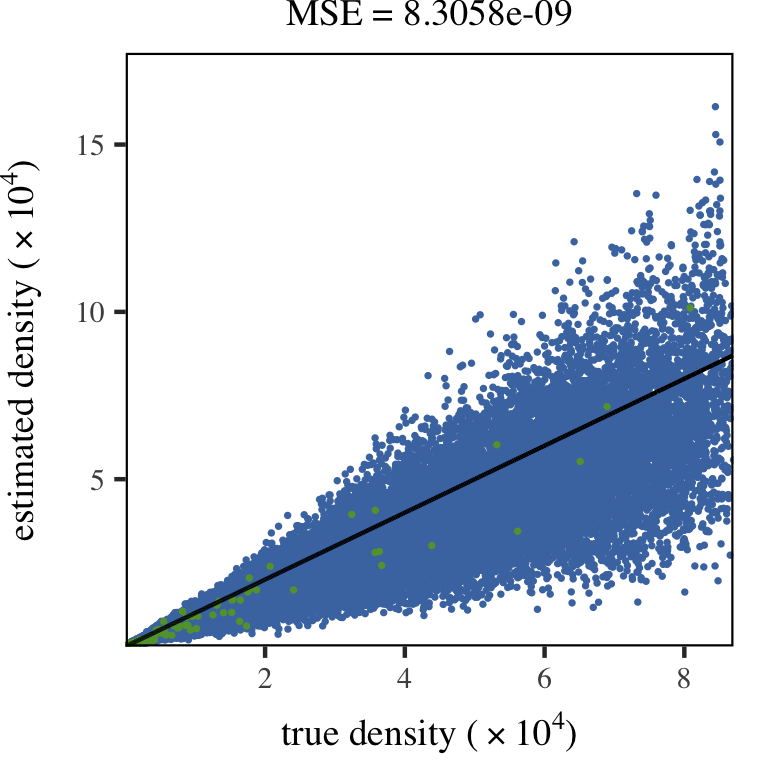
\includegraphics[keepaspectratio=true, width=\textwidth, height=0.23\textheight]{result/img/results_ferdosi_1_60000_mbe_silverman}
	\caption{Set \ferdosiOne, \mbe}
	\label{fig:results:singlesphere:mbe:ferdosi1}
\end{subfigure}
% Ferdosi 1 - SAMBE
\begin{subfigure}{0.3\textwidth}
	\centering
	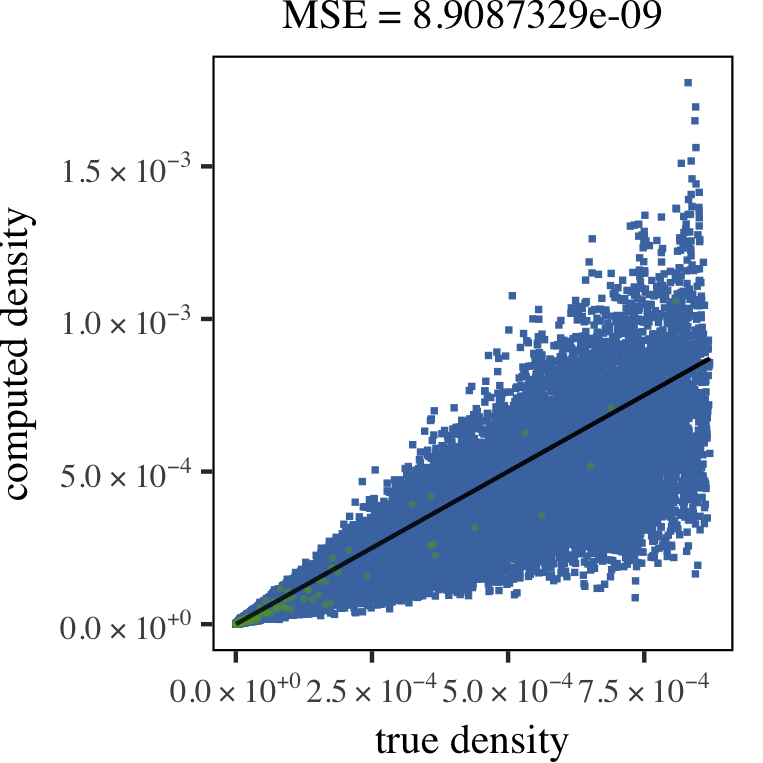
\includegraphics[keepaspectratio=true, width=\textwidth, height=0.23\textheight]{result/img/results_ferdosi_1_60000_sambe_silverman}
	\caption{Set \ferdosiOne, \sambe}
	\label{fig:results:singlesphere:sambe:ferdosi1}
\end{subfigure}
\subfigvspace
% Baakman 1	- MBE
\begin{subfigure}{0.3\textwidth}
	\centering
	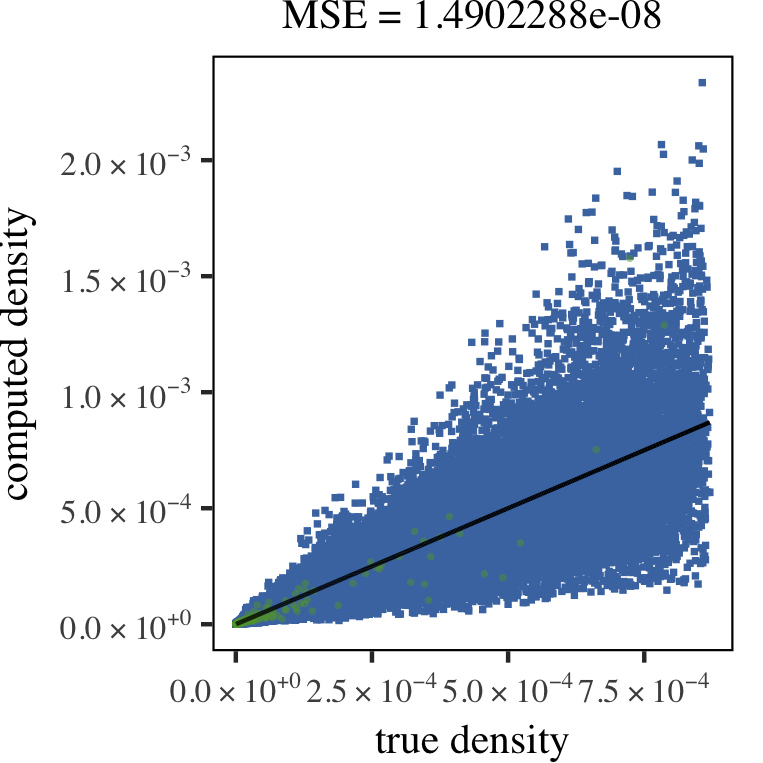
\includegraphics[keepaspectratio=true, width=\textwidth, height=0.23\textheight]{result/img/results_baakman_1_60000_mbe_silverman}
	\caption{Set \baakmanOne, \mbe}
	\label{fig:results:singlesphere:mbe:baakman1}
\end{subfigure}
% Baakman 1	- SAMBE
\begin{subfigure}{0.3\textwidth}
	\centering
	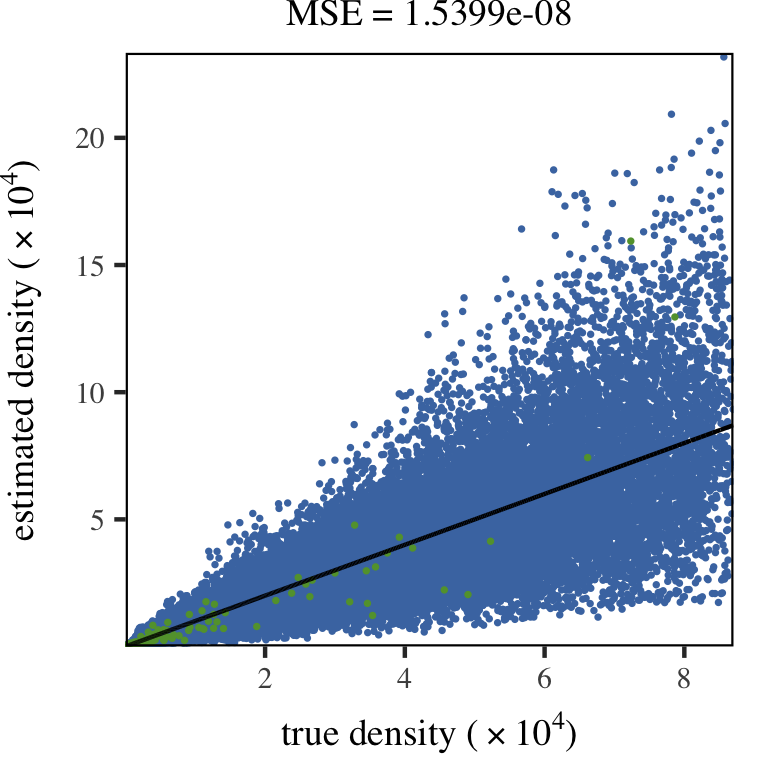
\includegraphics[keepaspectratio=true, width=\textwidth, height=0.23\textheight]{result/img/results_baakman_1_60000_sambe_silverman}
	\caption{Set \baakmanOne, \sambe}
	\label{fig:results:singlesphere:sambe:baakman1}
\end{subfigure}
\subfigvspace
% Baakman 4 - MBE
\begin{subfigure}{0.3\textwidth}
	\centering
	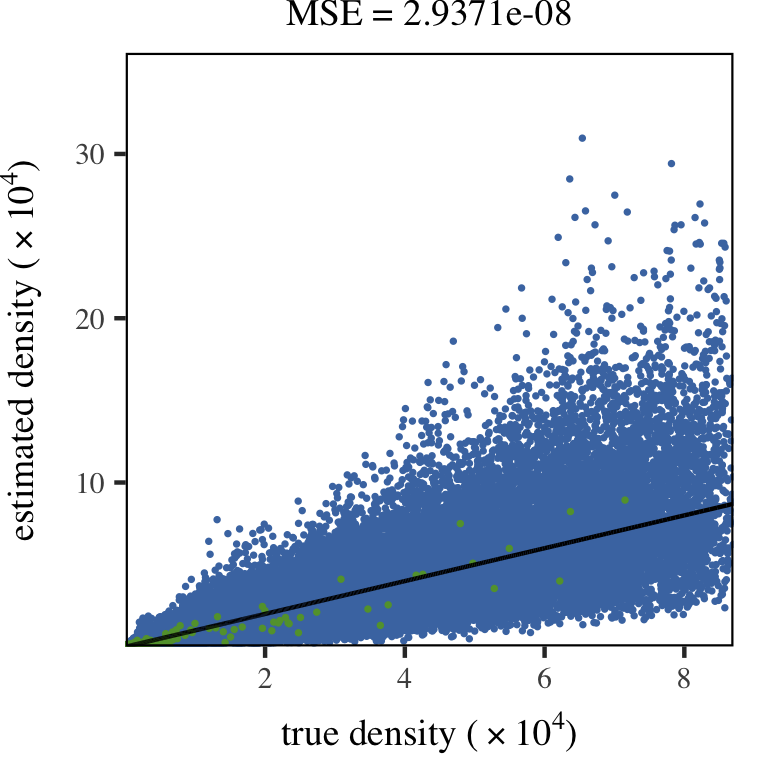
\includegraphics[keepaspectratio=true, width=\textwidth, height=0.23\textheight]{result/img/results_baakman_4_60000_mbe_silverman}
	\caption{Set \baakmanFour, \mbe}
	\label{fig:results:singlesphere:mbe:baakman4}
\end{subfigure}	
% Baakman 4 - SAMBE
\begin{subfigure}{0.3\textwidth}
	\centering
	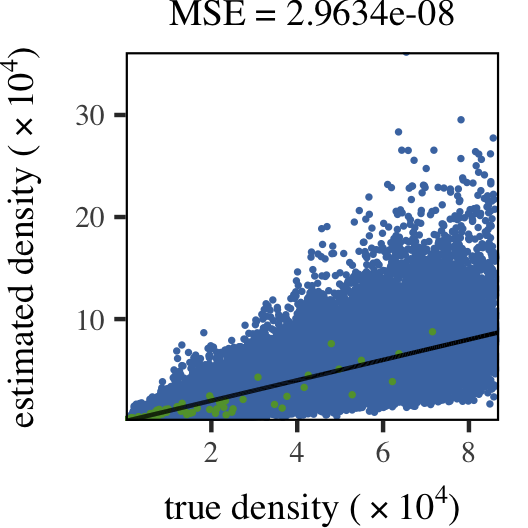
\includegraphics[keepaspectratio=true, width=\textwidth, height=0.23\textheight]{result/img/results_baakman_4_60000_sambe_silverman}
	\caption{Set \baakmanFour, \sambe}
	\label{fig:results:singlesphere:sambe:baakman4}
\end{subfigure}		
\subfigvspace
% Baakman 5 - MBE
\begin{subfigure}{0.3\textwidth}
	\centering
	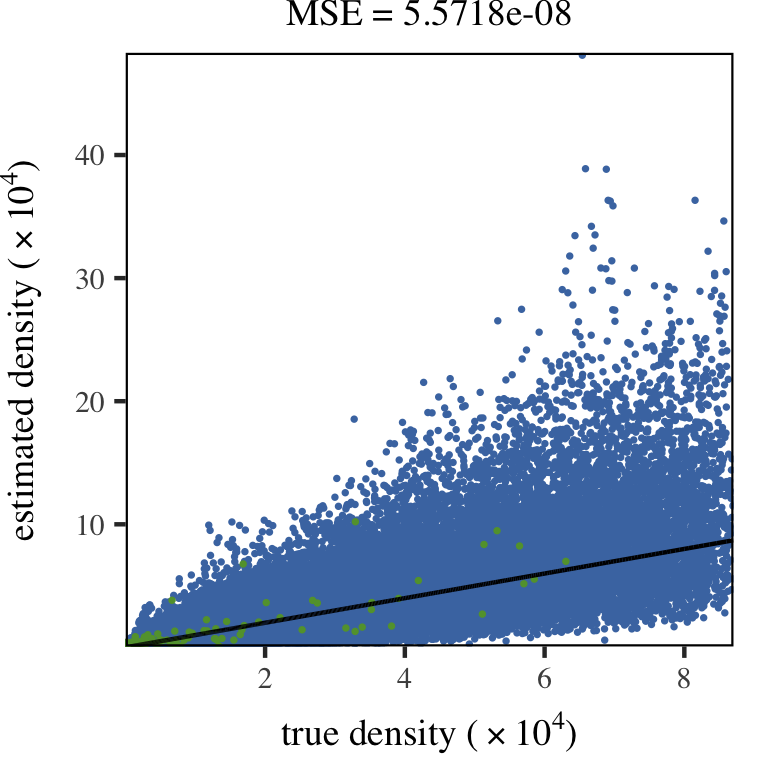
\includegraphics[keepaspectratio=true, width=\textwidth, height=0.23\textheight]{result/img/results_baakman_5_60000_mbe_silverman}
	\caption{Set \baakmanFive, \mbe}
	\label{fig:results:singlesphere:mbe:baakman5}
\end{subfigure}
% Baakman 5 - SAMBE
\begin{subfigure}{0.3\textwidth}
	\centering
	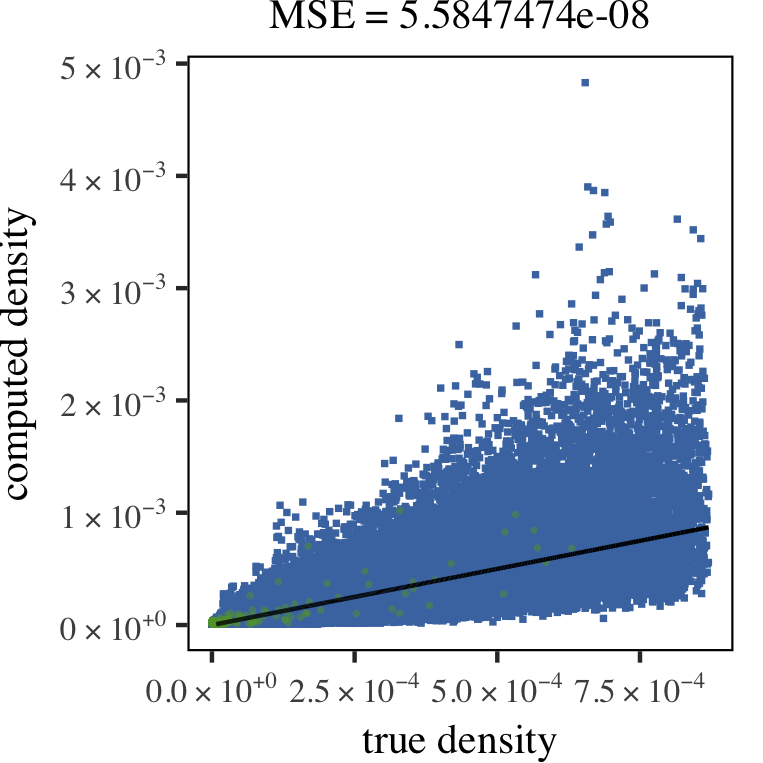
\includegraphics[keepaspectratio=true, width=\textwidth, height=0.23\textheight]{result/img/results_baakman_5_60000_sambe_silverman}
	\caption{Set \baakmanFive, \sambe}
	\label{fig:results:singlesphere:sambe:baakman5}
\end{subfigure}	
		\caption{The density as estimated by \mbe and \sambe as a function of the known density of data sets \ferdosiOne through \baakmanFive.}
		\label{fig:results:singleSphere:comparativePlots}
	\end{figure*}
	%
	This is confirmed by the visualization of the results in \cref{fig:results:singleSphere:comparativePlots} where hardly any difference is visible between \cref{fig:results:singlesphere:mbe:ferdosi1,fig:results:singlesphere:mbe:baakman1,fig:results:singlesphere:mbe:baakman4,fig:results:singlesphere:mbe:baakman5}, and \cref{fig:results:singlesphere:sambe:ferdosi1,fig:results:singlesphere:sambe:baakman1,fig:results:singlesphere:sambe:baakman4,fig:results:singlesphere:sambe:baakman5}, respectively.
		%Ferdosi 1
		Comparing the plots associated with data set \ferdosiOne, we find that the shape-adaptive estimator tends to overestimate densities more than the symmetric estimator if the Gaussian component is spherical.
		% Baakman 4
		Based on \cref{fig:results:singlesphere:mbe:baakman4,fig:results:singlesphere:sambe:baakman4} the same holds for set \baakmanFour.
	% Focus on components
	Comparing the performance within data sets between the two components showed no marked differences between the estimators between components.

%ANISOTROPY
	\begin{table}
		\centering
		%!TEX root = ../../paper.tex

% \sisetup{
% 	table-format=1.3e+1,
% 	scientific-notation=true, 
% 	table-number-alignment=center,
% }

% Mean and SD in single column
% \begin{tabular}{@{}c*{6}{c}@{}}
% \toprule
% ~				& Full Set 												& \legendComponentOne Gaussian 1						& \legendComponentTwo Gaussian 2						& \legendComponentThree Gaussian 3						& \legendComponentFour Gaussian 4					 	&  \legendComponentNoise Noise\\
% \midrule
% %
% \ferdosiTwo		& \meanSD{1.504005042371507e+00}{5.309582791641542e-01} & \meanSD{1.320121582169093e+00}{1.749869852989719e-01} & \meanSD{1.304784013773833e+00}{1.427734068384871e-01} & ~ 													& ~ 													& \meanSD{1.890276960903559e+00}{7.587403345342156e-01}\\
% \baakmanTwo 	& \meanSD{1.614716145373154e+00}{5.702499690627806e-01} & \meanSD{1.407377455694081e+00}{2.782480127488867e-01} & \meanSD{1.491043432778090e+00}{3.453168397321122e-01}	& ~ 													& ~ 													& \meanSD{11.948464282370670e+00}{7.826307984091438e-01}\\
% \ferdosiThree	& \meanSD{1.460357930082488e+00}{5.507084955708148e-01} & \meanSD{1.294023549845817e+00}{1.889517285607608e-01} & \meanSD{1.265946347671562e+00}{1.301150512342848e-01} & \meanSD{1.291829938425150e+00}{2.103396722315814e-01} & \meanSD{1.275739356043035e+00}{1.654855348814119e-01} & \meanSD{1.819950324176552e+00}{8.111641695146756e-01} \\
% \baakmanThree 	& \meanSD{1.532493079967588e+00}{5.713672219810757e-01} & \meanSD{1.314980484677339e+00}{2.190657831683435e-01} & \meanSD{1.487242917765238e+00}{3.393090417977690e-01} & \meanSD{1.291829938425150e+00}{2.103396722315814e-01} & \meanSD{1.396015162355687e+00}{2.851380764085146e-01} & \meanSD{1.854880861700560e+00}{8.195085323228068e-01}\\
% %
% \bottomrule
% \end{tabular}

\small
\sisetup{
	table-format=1.4,
	scientific-notation=fixed,
	table-number-alignment=center,
	fixed-exponent=0,
	round-mode=figures,
	round-precision=4
}


\begin{tabular}{@{}c*{12}{S}@{}}
\toprule
 				& \multicolumn{2}{c}{~} 						& \multicolumn{2}{c}{\legendComponentOne Gaussian 1} 	& \multicolumn{2}{c}{\legendComponentTwo Gaussian 2}	& \multicolumn{2}{c}{\legendComponentThree Gaussian 3}	& \multicolumn{2}{c}{\legendComponentFour Gaussian 4}	& \multicolumn{2}{c}{\legendComponentNoise Noise} \\
															  	\cmidrule(lr){4-5}							  				\cmidrule(lr){6-7}							  			\cmidrule(lr){8-9} 							  			\cmidrule(lr){10-11} 							  \cmidrule(lr){12-13}
~				& {\mean}				& {\SD}			& {\mean}				 & {\SD}			& {\mean}				 & {\SD}			 & {\mean}				& {\SD}			& {\mean}				& {\SD}			& {\mean}					& {\SD}\\ 			
\midrule
\ferdosiTwo		& 1.504005042371507e+00 & 5.309582791641542e-01 & 1.320121582169093e+00 & 1.749869852989719e-01 & 1.304784013773833e+00 & 1.427734068384871e-01 &  						&  						& 	 					&  							& 1.890276960903559e+00 	& 7.587403345342156e-01\\
\baakmanTwo 	& 1.614716145373154e+00 & 5.702499690627806e-01 & 1.407377455694081e+00 & 2.782480127488867e-01 & 1.491043432778090e+00 & 3.453168397321122e-01 &  						&  						& 	 					&  							& 1.948464282370670e+00 	& 7.826307984091438e-01\\
\ferdosiThree 	& 1.460357930082488e+00 & 5.507084955708148e-01 & 1.294023549845817e+00 & 1.889517285607608e-01 & 1.265946347671562e+00 & 1.301150512342848e-01 & 1.291829938425150e+00 & 2.103396722315814e-01 & 1.275739356043035e+00 & 1.654855348814119e-01 	& 1.819950324176552e+00 	& 8.111641695146756e-01 \\
\baakmanThree 	& 1.532493079967588e+00 & 5.713672219810757e-01 & 1.314980484677339e+00 & 2.190657831683435e-01 & 1.487242917765238e+00 & 3.393090417977690e-01 & 1.291829938425150e+00 & 2.103396722315814e-01 & 1.396015162355687e+00 & 2.851380764085146e-01 	& 1.854880861700560e+00 	& 8.195085323228068e-01\\
\bottomrule
\end{tabular}
		\caption{The mean (\mean) and the standard deviation (\SD) of the anisotropy of the kernels used for the data sets with a single Gaussian.}
		\label{tab:results:singleSphere:anisotropy}
	\end{table}
	%
	% General
	\Cref{tab:results:singleSphere:anisotropy} presents the mean and the standard deviation of the anisotropy of the kernels used for the different data sets. Comparing the means we find a positive correlation between the anisotropy of the Gaussian component of the data set and the mean anisotropy of the kernels. The same positive correlation can be observed for the standard deviation. Furthermore as the anisotropy of the Gaussian component increases, the anisotropy of the kernels associated with points sampled from the uniform random background rises.
	% Focus on components
	Reviewing these statistics of the components of the data sets reveals that the increase in average anisotropy is primarily caused by an increase in anisotropy of kernels of points sampled from the Gaussian component. The mean anisotropy of the background component stays relatively constant. Furthermore as the Gaussian component is more anisotropic the variation in anisotropy of the kernels increases.

%Summary
To summarize; in spite of differences in anisotropy of the used kernels we have observed very few differences between the two estimators. Using shape-adaptive kernels did not yield the expected gain in performance. We did find the hypothesized influence of the anisotropy of the Gaussian components on the shape of the kernels. Furthermore the kernels associated with points sampled from the background are more anisotropic than those belonging to points drawn from the Gaussian distribution.


\textcite{ferdosi2011comparison} found that the \mbe resulted in lower integrated squared errors if fewer Gaussian distributions were present in the data sets. Since the presented data sets are comparable to those used by \citeauthor{ferdosi2011comparison} we expect to find the same influence on the \mse.
